\section{What is ontology?}

The term ontology is used both in computer sciences and philosophy, but not with the exact same purpose. Both are areas of study that focus on representing entities, ideas and events and their relationships and properties. The difference lies in the fact that computer science mostly studies how to create ontologies (ontology engineering) about specific domains and to use them in computer systems \citep{gruber2009ontology}. Whilst philosophy focus on understanding the nature of ontology, of the being and what exists, that is studying more abstract subjects of ontology and also providing classification for ontological concepts \citep{guizzardi_ontological_2005}.

In regards to ontology engineering there are different types of ontology according to their level of generalization. The most generic type is \textit{top-level ontologies} which describe concepts that are independent of a problem or domain, as such it defines concepts like events, actions, objects, spaces, time, etc. Next there is the specialization of the top-level ontology, which are \textit{domain ontologies} or \textit{task ontologies}, respectively, when describing a domain or problem. Such ontologies are presented by specifying the concepts presented in a top-level ontology, which means they present the vocabulary of their subject domain or problem. At last there is \textit{application ontologies} which merge a domain ontology and a task ontology, it presents concepts which relate to a specific problem of a domain \citep{guarino1998ontoformal}.

The objective for creating an ontology is, in computer science, mainly to use them in an application. There are three areas that are mostly responsible for the demand for such applications of ontology, database and information systems, software engineering and artificial intelligence \citep{smith2001ontology}. For database and information systems ontology is mostly used as a theoretical basis to better model reality or to evaluate existing models. To software engineering ontology became very important as a tool to be used in domain engineering. The study of ontology became important in addressing how intelligent systems acquire and model knowledge.

\subsection{Modeling languages and conceptualization}

In \cite{guizzardi_ontological_2005} there is an important clarification about some concepts surrounding a model. First of all, a model in and by itself is an abstract entity as it is an abstraction of a given subject. The concrete form of a model is given by a specification, which is a set of concepts, relationships and rules that translate the model. The specification need to be written using a modeling language, that has the syntax and vocabulary needed to express the specification. A conceptualization is an abstraction of the world's concepts, that is, it contains the ideas and possibilities of the world. This is what defines the modeling language, giving fruition to its vocabulary and meaning to the syntax. The model needs a fitting conceptualization to be created. So the choice of specification, modeling language and conceptualization are heavily entwined with the idealized model.

In the diagram of \autoref{fig:model_diag} there is a visual representation of those concepts:

%Conceptuaization diagram
\begin{figure}[ht]
\centering

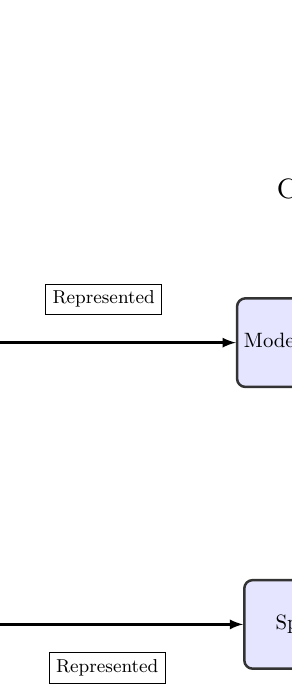
\begin{tikzpicture}[squarednode/.style={rectangle, 
					rounded corners, 
					very thick,
 					minimum width=3cm,
					minimum height=1.5cm,
					draw=black!80, 
					fill=red!10},
					squarednode2/.style={rectangle, 
					rounded corners, 
					very thick,
 					minimum width=3cm,
					minimum height=1.5cm,
					draw=black!80, 
					fill=blue!10}
					]
					
% To reduce all image, transform canvas
% forgets about image size, so 
% we need a bounding box
% This is lame, but works with Eduardo Thesis´s image (now black and white for elegance)

% don´t ask me about theses limits
% I just tried until I found which ones
%workded
\useasboundingbox (3,-4) rectangle (6,4);
\scope[transform canvas={scale=.75}]
         % Your actual drawing


%model nodes
\node[squarednode]  (concept) [anchor = west]{Conceptualization};
\node[squarednode2]  (mlang) [right of = concept, node distance=6cm, anchor=west] {Modeling Language};
\node[squarednode]  (model) [below of = concept, node distance=4cm, anchor=north] {Model};
\node[squarednode2]  (spec) [below of = mlang, node distance=4cm, anchor=north] {Specification};

% Arrows
\path[-latex, double, black, very thick] (concept.south) edge  coordinate[midway](c_to_m) (model.north);

\path[-latex, double, black, very thick] (mlang.south) edge  coordinate[midway](ml_to_s) (spec.north);

\path[-latex, double, black, very thick] (concept.east) edge  coordinate[midway](ml_to_c) (mlang.west);

\path[-latex, double, black, very thick] (model.east) edge  coordinate[midway](m_to_s) (spec.west);


\node [draw] (ml_to_cleg) [above of = ml_to_c, align=center, node distance=1cm, anchor=north]{\small Represented};

\node [draw] (m_to_sleg) [below of = m_to_s, align=center, node distance=1cm, anchor=south]{\small Represented};

\node [draw] (m_to_cleg) [left of = c_to_m, align=center, node distance=0.5cm, anchor=east]{\small Compose};

\node [draw] (ml_to_sleg) [right of = ml_to_s, align=center, node distance=0.5cm, anchor=west]{\small Compose};

\node (abs) [scale = 1.5, above of = concept, align=center, node distance=1.5cm, anchor=south]{\small Abstract};

\node (conc) [scale = 1.5, above of = mlang, align=center, node distance=1.5cm, anchor=south]{\small Concrete};

%\draw [dashed,<-,very thick](designerPathnew.north) |- (designerLegend.east);

    \endscope
\end{tikzpicture}
\caption{Modeling Diagram \citep{guizzardi_ontological_2005}}
\label{fig:model_diag}
\end{figure}

It is duly noted that the distinction made is between abstract and concrete ideas. The concrete are defined as such because they have a material form with which one can interact. On the other hand the abstract concepts withhold the meaning conveyed by the concrete entities.

From the perspective of this work the model is the objective, so we center it on the interpretation of the diagram. That said, the model is an abstraction of a particular idea which resides in the world. So although it is the conceptualization that allows to compose a model, the target models need to have compatible conceptualization. An example, one cannot correctly create a model of soccer games using a conceptualization of the politics. This is called ``conceptualization appropriateness '' \cite{guizzardi_ontological_2005}.

The conceptualization comes with a modeling language to express its ideas. With this language it is possible to create a specification that represent a given model. But this specification must be according to the abstract model, otherwise it is no specification at all. 

Lastly, it should be noted that the relationships between the concepts are double-sided. Whilst a model is represented by a specification it is also interpreted from it. And while a conceptualization is used to compose a model, the model is an instance of that conceptualization.

Perhaps more important than these ideas is how they limit each other. And thus they need to be carefully accounted when modeling. This work thus abide to the conceptualization and modeling language provided by the Universal Foundational Ontology and OntoUML.